\documentclass{article}
\usepackage[utf8]{inputenc}
\usepackage{amsmath}
\usepackage[margin=1cm]{geometry}
\usepackage[english]{babel} % English language/hyphenation
\usepackage{amsmath,amsthm,amssymb}
\usepackage{setspace} %for Double Spacing
\usepackage{breqn}
%\usepackage{enumitem}
%\setitemize{nolistsep}
\usepackage{enumerate}
\usepackage{multicol}
\usepackage{pgfplots}


\theoremstyle{definition}
\newtheorem{theorem}{Exercise}[section]

\theoremstyle{remark}
\newtheorem*{claim}{Claim}

\newcommand{\R}{\mathbb{R}}
\newcommand{\Z}{\mathbb{Z}}
\newcommand{\N}{\mathbb{N}}
\newcommand{\inv}[1]{#1^{-1}}
\setcounter{section}{5}

\doublespacing
%\onehalfspacing
\begin{document}
	\begin{flushright}
		Moshe Mason Rubin\\MATH 330 Homework \#6\\10 October 2016
	\end{flushright}
	
	\setcounter{theorem}{7}
	\begin{theorem}
		Show that $A_{10}$ contains an element of order $15$.
	\end{theorem}
	\begin{proof}
		Consider $\sigma\in A_{10}\subset S_{10}$ given by $\sigma=(12345)(678)$, the product of two disjoint cycles. Then $\sigma\in A_{10}$ as $\sigma$ is the product of two even permutations and Theorem 5.7 states $A_{10}$ is a sub-group of $S_{10}$, therefore closed. Notice $\inv{(12345)}=(12345)^4$ and $\inv{(678)}=(678)^2$, and clearly $\inv{(12345)}\not=(678)^n$ and $\inv{(678)}\not=(12345)^m$ for any $(n,m)\in\Z^2$. Because $|A_{10}|=\frac{10!}{2}$ is finite, $|\sigma|\not=\infty$ as $\sigma^n\in A_{10}$ for all $n\in\Z$ by Theorem 5.7 that $A_n$ is a sub-group of $S_n$. Then
		\begin{dmath*}
			\sigma^{15} = \left[(12345)(678)\right]^{15} = (12345)^{15}(678)^{15} \condition[]{by Proposition 5.2 (that disjoint cycles commute) and Theorem 3.8.3} = \left[(12345)^5\right]^3\left[(678)^3\right]^5 \condition[]{by Theorem 3.8.2} = \left(id\right)^3\left(id\right)^5= id
		\end{dmath*} So $\sigma=(12345)(678)\in A_{10}$ is an element of $A_{10}$ of order $15$. 
	\end{proof}

	\setcounter{theorem}{12}
	\begin{theorem}
		Let $\sigma=\sigma_1\cdots\sigma_m\in S_n$ be the product of disjoint cycles. Prove that the order of $\sigma$ is the least common multiple of the lengths of the cycles $\sigma_1,\ldots,\sigma_m$.
	\end{theorem}
	\begin{proof}
		Let $|\sigma|=k$. So 
		\begin{dmath*}
			\sigma^k = \left(\sigma_1\cdots\sigma_m\right)^k = \sigma_1^k\cdots\sigma_m^k \condition[]{by Proposition 5.2 (that disjoint cycles commute) and Theorem 3.8.3} = id \condition[]{because $\sigma^k=id$ as $|\sigma|=k$}
		\end{dmath*}
		So $\sigma_i^k=id$ for $i\in\left(\left[1,m\right]\cap\Z\right)$. So if So $\sigma_i^k=id$ then $k$ must be a common multiple of the length of each $\sigma_i$. So the smallest $k$ (that is, the order of $\sigma$) must be equal to the least common divisor of lengths of $\sigma_1,\ldots\sigma_m$ by definition of least common multiple. 
	\end{proof}


	\setcounter{theorem}{15}
	\begin{theorem}
		Find all group of rigid motions of a tetrahedron. Show that this is the same group as $A_4$.
	\end{theorem}
	\begin{proof} \hfill\\
		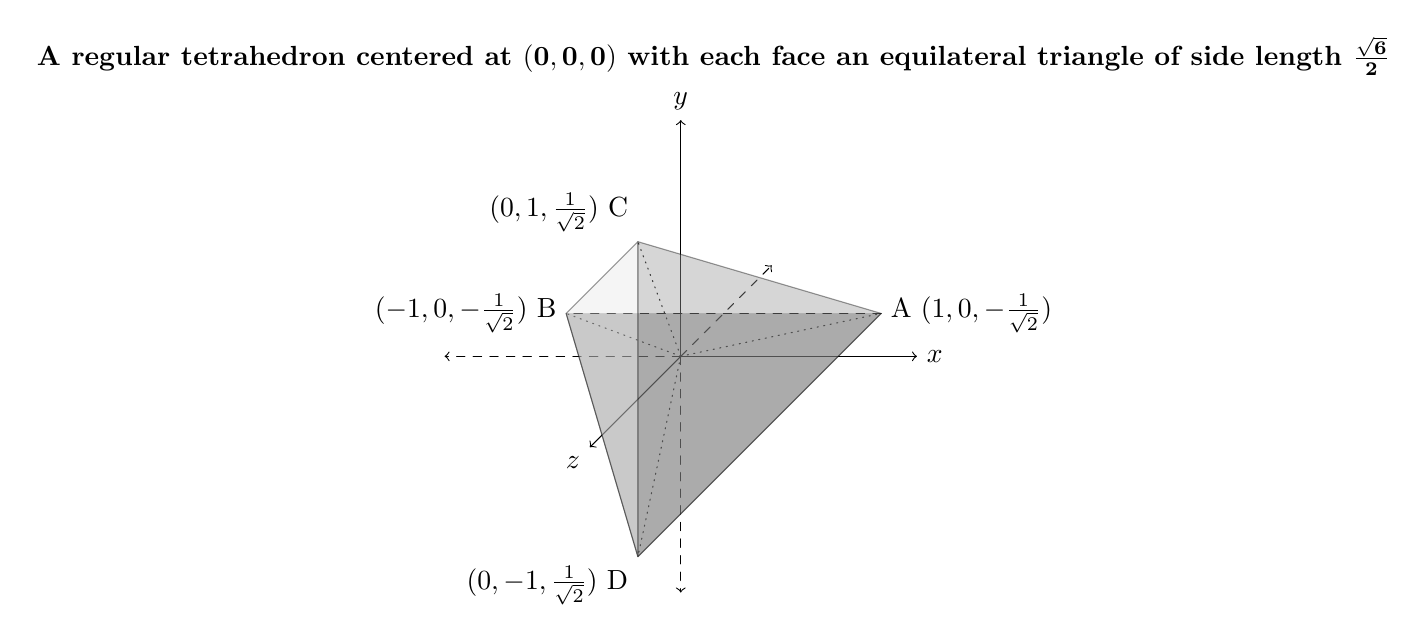
\begin{tikzpicture}[line join = round, line cap = round]
		%\addplot [title=bleh]
		\pgfmathsetmacro{\factor}{1/sqrt(2)};
		\coordinate [label={right:{A $(1,0,-\frac{1}{\sqrt{2}})$}}] (A) at (2,0,-2*\factor);
		\coordinate [label=left:{$(-1,0,-\frac{1}{\sqrt{2}})$ B}] (B) at (-2,0,-2*\factor);
		\coordinate [label=above left:{$(0,1,\frac{1}{\sqrt{2}})$ C}] (C) at (0,2,2*\factor);
		\coordinate [label=below left:{$(0,-1,\frac{1}{\sqrt{2}})$ D}] (D) at (0,-2,2*\factor);
		
		\draw[->] (0,0) -- (3,0,0) node[right] {$x$};
		\draw[->] (0,0) -- (0,3,0) node[above] {$y$};
		\draw[->] (0,0) -- (0,0,3) node[below left] {$z$};
		\draw[dashed,->] (0,0) -- (-3,0,0) node[left] {}; 
		\draw[dashed,->] (0,0) -- (0,-3,0) node[below] {}; 
		\draw[dashed,->] (0,0) -- (0,0,-3) node[above right] {}; 
		\foreach \i in {A,B,C,D}
		\draw[dotted] (0,0,0)--(\i);
		\draw[-, fill=black!70, opacity=.4] (A)--(D)--(B);%--cycle;
		\draw[dashed, fill=black!70] (A) -- (B);
		\draw[-, fill=black!40, opacity=.4] (A) --(D)--(C)--cycle;
		\draw[-, fill=black!10, opacity=.4] (B)--(D)--(C)--cycle;
		
		% title
		\node[align=center,font=\bfseries, yshift=1em] (title) 
		at (current bounding box.north)
		{A  regular tetrahedron centered at $\mathbf{(0,0,0)}$ with each face an equilateral triangle of side length $\mathbf{\frac{\sqrt{6}}{2}}$};
		
		\end{tikzpicture}\\
		Consider the position of face $ACD\to A'C'D'$ for each rigid motion of the tetrahedron. The point $A$ may assume $4$ distinct locations. Once $A$ is fixed, $C$ may assume one of $3$ remaining distinct locations. Once $A$ and $C$ are chosen, $D$ may assume only $1$ distinct location. So the order is $4\times3\times1=12$. The group of rigid rotations is given by $\rho_A = \left(\begin{smallmatrix}
		A & B & C & D \\ 
		A & D & B & C
		\end{smallmatrix} \right)$, $\rho_A^2 = \left(\begin{smallmatrix}
		A & B & C & D \\ 
		A & C & D & B
		\end{smallmatrix} \right)$, $\rho_B=\left(\begin{smallmatrix}
		A & B & C & D \\ 
		C & B & D & A
		\end{smallmatrix} \right)$, $\rho_B^2=\left(\begin{smallmatrix}
		A & B & C & D \\ 
		D & B & A & C
		\end{smallmatrix} \right)$, $\rho_C=\left(\begin{smallmatrix}
		A & B & C & D \\ 
		B & D & C & A
		\end{smallmatrix} \right)$, $\rho_C^2=\left(\begin{smallmatrix}
		A & B & C & D \\ 
		D & A & C & B
		\end{smallmatrix} \right)$, $\rho_D=\left(\begin{smallmatrix}
		A & B & C & D \\ 
		C & A & B & D
		\end{smallmatrix} \right)$, $\rho_D^2=\left(\begin{smallmatrix}
		A & B & C & D \\ 
		B & C & A & D
		\end{smallmatrix} \right)$, $\rho_{AB,BC} = \left(\begin{smallmatrix}
		A & B & C & D \\ 
		B & A & D & C
		\end{smallmatrix} \right)$, $\rho_{AC,BD} = \left(\begin{smallmatrix}
		A & B & C & D \\ 
		C & D & A & B
		\end{smallmatrix} \right)$, $\rho_{AD,BC} = \left(\begin{smallmatrix}
		A & B & C & D \\ 
		D & C & B & A
		\end{smallmatrix} \right)$, and $id = \left(\begin{smallmatrix}
		A & B & C & D \\ 
		A & B & C & D
		\end{smallmatrix} \right)$. By Proposition 5.8, $A_4\subset S_4$ is of order $\frac{4!}{2}=12$ and $A_4$ is given by 
		\begin{dmath*}
			A_4 = \left\{id,(12)(13),(12)(14),(12)(34),(13)(12),(13)(14),(13)(24),(14)(12),(14)(13),(14)(23),(23)(24),(24)(23)\right\} \condition[]{by definition} = \left\{(24)(23),(23)(24),(14)(13),(13)(14),(14)(12),(12)(14),(13)(12),(12)(13),(12)(34),(13)(34),(14)(23), id\right\} \condition[]{by reordering}= \left\{(234),(243),(134),(143),(124),(142),(123),(132),(12)(34),(13)(24),(14)(23),id\right\} \condition[]{as $(a_ia_k)(a_ia_j) = \left(a_ia_ka_j\right)$.}
		\end{dmath*} Notice this matches the set $A_4$ as listed in Chapter 5, \textbf{Example 8.}\\ 
		Since the order of the rigid motions of a tetrahedron equals the order of $A_4$, to show that the two groups are equivalent we must show that every rigid motion of a tetrahedron is the product even number of permutations. Label $A, B, C, D$ as $1,2,3,4$ respectively. Then 
		\begin{multicols}{4}\noindent
		\begin{itemize}
			\item $(234)$ corresponds to $\rho_A$ ($(243)$ to $\rho_A^2$)
			\item $(134)$ corresponds to $\rho_B$ ($(143)$ to $\rho_B^2$)
			\item $(124)$ corresponds to $\rho_C$ ($(142)$ to $\rho_C^2$)
			\item $(123)$ corresponds to $\rho_D$ ($(132)$ to $\rho_D^2$)
			\item $(12)(34)$ corresponds to $\rho_{AB,BC}$
			\item $(13)(24)$ corresponds to $\rho_{AC,BD}$
			\item $(14)(23)$ corresponds to $\rho_{AD,BC}$
			\item The identity $id$ corresponds to itself
		\end{itemize}
		\end{multicols}\noindent
		Notice every rigid motion of is the product of an even number of permutations as for each $x\in\left\{\text{group of rigid motions of a tetrahedron}\right\}$, $x\in A_{4}$. So the group of rigid motions of a tetrahedron is the same as $A_{4}$ as
		\begin{dmath*}
			\left\{\text{group of rigid motions of a tetrahedron}\right\} = \left\{\rho_A, \rho_A^2, \rho_B, \rho_B^2,\rho_C, \rho_C^2, \rho_D, \rho_D^2, \rho_{\left((AB)(BC)\right)}, \rho_{\left((AC)(BD)\right)},\rho_{\left((AD)(BC)\right)}\right\} \condition[]{from way above} = \left\{(234),(243),(134),(143),(124),(142),(123),(132),(12)(34),(13)(24),(14)(23),id\right\} \condition[]{from above} = \left\{id,(12)(34),(13)(24),(14)(23),(123),(132),(124), (142), (134), (143), (234), (243)\right\} \condition[]{by reordering} = A_4 \condition[]{as listed in Chapter 5, \textbf{Example 8.} and above}\hfill\qedhere
		\end{dmath*}
	\end{proof}


	\setcounter{theorem}{18}
	\begin{theorem}
		Prove that $D_n$ is non-abelian for $n\geq3$.
	\end{theorem}
	\begin{proof}
		By Theorem 5.10, we know that the group $D_n$ consists of all products of the two elements $r$ and $s$ satisfying the relations
		\begin{dmath*}
			{r^n=id}\\
			{s^2=id}\\
			{srs=\inv{r}}
		\end{dmath*} for $n\geq 3$.\\
		Let $n\geq3$ and label $r,s$ such that $r^n=id$ and $s^2=id$, which is certainly possible by Theorem 5.10. Now assume for a contradiction of $D_n$ is abelian. Then 
		\begin{dmath*}
			srs \hiderel{=} (sr)s = (rs)s \condition[]{by assumption that $D_3$ is abelian} = r(ss) \hiderel{=} rs^2 \condition[]{by associativity of elements in $D_n$ as $D_n$ is a sub-group of $S_n$ by Theorem 5.9} = r(id) \condition[]{by Theorem 5.15 and chose of $s\in D_n$} = r 
		\end{dmath*} However $srs=r$ is a contradiction to Theorem 5.10 that $srs=\inv{r}$ as this would imply 
		\begin{dmath*}
			r\inv{r} \hiderel{=} id \implies r(srs) \hiderel{=} id \condition[]{by Theorem 5.10} \implies r(r) \hiderel{=} id \condition[]{by calculation above that $srs=r$} \implies r^2 \hiderel{=} id
		\end{dmath*} and $r^2=id$ cannot happen for $r\in D_n$ for $n\geq3$ as $r$ is necessarily of order $n$ and $2<n$. So our original assumption that $D_n$ is abelian must be false, so $D_n$ must be non-abelian for $n\geq 3$.
	\end{proof}
	
	
	\setcounter{theorem}{22}
	\begin{theorem}
		If $\sigma$ is a cycle of odd length, prove that $\sigma^2$ is also a cycle.
	\end{theorem}
	\begin{proof}
		Let $\sigma = \left(\sigma_1,\ldots,\sigma_k\right)$ for some odd integer $k$. Then $\sigma$ may be written as $\sigma=\left(\sigma_1\sigma_k\right)\left(\sigma_1\sigma_{k-1}\right)\cdots\left(\sigma_1\sigma_3\right)\left(\sigma_1\sigma_2\right)$, a finite product of transpositions. Then 
		\begin{dmath*}
			\sigma^2 = \left(\left(\sigma_1\sigma_k\right)\left(\sigma_1\sigma_{k-1}\right)\cdots\left(\sigma_1\sigma_3\right)\left(\sigma_1\sigma_2\right)\right)^2 = \left[\left(\sigma_1\sigma_k\right)\left(\sigma_1\sigma_{k-1}\right)\cdots\left(\sigma_1\sigma_3\right)\left(\sigma_1\sigma_2\right)\right]\left[\left(\sigma_1\sigma_k\right)\left(\sigma_1\sigma_{k-1}\right)\cdots\left(\sigma_1\sigma_3\right)\left(\sigma_1\sigma_2\right)\right] \condition[]{by definition of exponentiation}
		\end{dmath*} Then $\sigma^2$ is given by $\sigma^2\left(\sigma_\ell\right) = \sigma \left(\sigma\left(\sigma_{\ell}\right)\right) = \sigma\left(\sigma_{\ell+1}\right) = \sigma_{\ell+2}$ for $\ell=1,2,\ldots,k-2$. So $\sigma^2:\sigma_1\mapsto \sigma_3$, and $\sigma^2:\sigma_3\mapsto \sigma_5$, and eventually we will arrive at $\sigma^2:\sigma_{k-2}\mapsto\sigma_{k}$ as  $k$ is an odd number. Then $\sigma^2\left(\sigma_k\right)=\sigma\left(\sigma_1\right)=\sigma_2$. $\sigma^2\left(\sigma_\ell\right) = \sigma \left(\sigma\left(\sigma_{\ell}\right)\right) = \sigma\left(\sigma_{\ell+1}\right) = \sigma_{\ell+2}$ for $\ell=1,2,\ldots,k-2$. So $\sigma^2:\sigma_2\mapsto \sigma_4$, and $\sigma^2:\sigma_4\mapsto \sigma_6$, and eventually we will arrive at $\sigma^2:\sigma_{k-3}\mapsto\sigma_{k-1}$ as  $k$ is an odd number so $k-3$ is even. Then $\sigma_{k-1}\mapsto \sigma_1$ as $\sigma_1\mapsto\sigma_3$ as before. So $\sigma^2=\left(\sigma_3,\sigma_5,\ldots,\sigma_{k-2},\sigma_k,\sigma_2,\sigma_4,\ldots,\sigma_{k-1},\sigma_1\right)$ is a cycle.
	\end{proof}


	\setcounter{theorem}{25}
	\begin{theorem}
		Prove that any element in $S_n$ can be written as a finite product of the following permutations.
		\begin{multicols}{3}
		\begin{enumerate}[(a)]%[label=\arabic{enumi}.\arabic*.]
			\item $(12),(13),\ldots,(1n)$
			\item $(12),(23),\ldots,\left(n-1,n\right)$
			\item $(12),(12\ldots n)$
		\end{enumerate}
		\end{multicols}
	\end{theorem}
	\begin{proof} Let $\sigma\in S_n$. 
		\begin{enumerate} [(a)]
			\item Then by Theorem 5.3, $\sigma$ can be written as the product of disjoint cycles $\sigma=a_1a_2\cdots a_k$. For $i=1,\ldots k$, let $a_i=\left(\alpha_{i_1},\ldots,\alpha_{i_\ell}\right)$. Then $a_i:\alpha_{i_m}\mapsto\alpha_{i_{m+1}}$ for $m=1,\ldots,\ell-1$ and $a_i:\alpha_{i_\ell}\mapsto\alpha_1$. Consider $a'_i=(\alpha_{i_1}a_{i_\ell})(a_{i_1}a_{i_{\ell-1}})\cdots(a_{i_1}a_{i_3})(a_{i_1}a_{i_2})$, which is a product of $(12),(13),\ldots,(1n)$. Then $a_i':\alpha_{i_m}\mapsto\alpha_{i_{m+1}}$ for $m=1,\ldots,\ell-1$ and $a_i':\alpha_{i_\ell}\mapsto\alpha_1$. So $a_i=a'_i$ for all $i$. So 
			\begin{dmath*}
				\sigma = a_1a_2\cdots a_k = a_1'a_2'\cdots a_k' \condition[]{as $a_i=a'_i$} = \left((a_{1_1}a_{1_\ell})\cdots(a_{1_1}a_{1_2})\right)\left((a_{2_1}a_{2_\ell})\cdots(a_{2_1}a_{2_2})\right)\cdots \left((a_{k_1}a_{k_\ell})\cdots(a_{k_1}a_{k_2})\right)
			\end{dmath*}which is a product of $(12),(13),\ldots,(1n)$\qedhere
		\end{enumerate}
	\end{proof}
	
	
	\setcounter{section}{6}
	\setcounter{theorem}{0}
	\begin{theorem}
		Suppose that $G$ is a finite group with an element $g$ of order $5$ and an element $h$ of order $7$. Why must $|G|\geq35$?
	\end{theorem}
	\begin{proof}
		Let $g=(g_1g_2g_3g_4g_5)$ and $h=(h_1h_2h_3h_4h_5h_6h_7)$. By Corollary 6.6, the orders of $g$ and $h$, (5 and 7 respectively) must divide the number of elements in $G$, so $|G|$ is $35$ at least, or larger. 
	\end{proof}
	
	
	\setcounter{theorem}{2}
	\begin{theorem}
		Prove or disprove: Every sub-group of the integers has finite index.
	\end{theorem}
	\begin{proof}
		This is false. Let $H=\left\{1\right\}$. Then $H$ is a sub-group of $\Z$ and $\left[\Z:H\right]=\#\mathcal{L}_H=\#\left\{g\cdot 1:g\in\Z\right\}=\infty$
	\end{proof}


	\setcounter{theorem}{4}
	\begin{theorem} List the left and right co-sets of the sub-groups in each of the following.
		\begin{multicols}{4}
		\begin{enumerate}[(a)]
			\item $\left\langle8\right\rangle$ in $\Z_{24}$
			\item $\left\langle3\right\rangle$ in $U\left(8\right)$
			\setcounter{enumi}{3}
			\item $A_4$ in $S_4$ \addtocounter{enumi}{1}
			\item $D_4$ in $S_4$
		\end{enumerate}
		\end{multicols}
	\end{theorem}
	\begin{proof}[Solution]\hfill
		\begin{enumerate}[(a)]
			\item The left and right co-sets of $\left\langle8\right\rangle$ in $\Z_{24}$ are the same as addition is commutative in $\Z_{24}$. So the left and right co-set are 
			\begin{align*}
			0+&\left\langle8\right\rangle	& =&	&	8+&\left\langle8\right\rangle	&=&&	16+&\left\langle8\right\rangle	&=&	&	\left\{0,8,16\right\}\\
			1+&\left\langle8\right\rangle	&=&	&	9+&\left\langle8\right\rangle	&=&	&	17+&\left\langle8\right\rangle	&=&	&	\left\{1,9,17\right\}\\
			2+&\left\langle8\right\rangle	&=&	&	10+&\left\langle8\right\rangle	&=&	&	18+&\left\langle8\right\rangle	&=&	&	\left\{2,10,18\right\}\\
			3+&\left\langle8\right\rangle	&=&	&	11+&\left\langle8\right\rangle	&=&	&	19+&\left\langle8\right\rangle	&=&	&	\left\{3,11,19\right\}\\
			4+&\left\langle8\right\rangle	&=&	&	12+&\left\langle8\right\rangle	&=&	&	20+&\left\langle8\right\rangle	&=&	&	\left\{4,12,20\right\}\\
			5+&\left\langle8\right\rangle	&=&	&	13+&\left\langle8\right\rangle	&=&	&	21+&\left\langle8\right\rangle	&=&	&	\left\{5,13,21\right\}\\
			6+&\left\langle8\right\rangle	&=&	&	14+&\left\langle8\right\rangle	&=&	&	22+&\left\langle8\right\rangle	&=&	&	\left\{6,14,22\right\}\\
			7+&\left\langle8\right\rangle	&=&	&	15+&\left\langle8\right\rangle	&=&	&	23+&\left\langle8\right\rangle	&=&	&	\left\{6,14,22\right\}\\
			\end{align*}
			\item The left and right co-sets of $\left\langle3\right\rangle$ in $U(8)$ are the same as multiplication is commutative in $\Z_8$. $U(8)=\left\{1,3,5,7\right\}$ and $\left\langle3\right\rangle=\left\{1,3\right\}$, so the left and right co-sets are:
			\begin{dmath*}
				{1\cdot\left\{3,1\right\}=\left\{3,1\right\}}\\
				{3\cdot\left\{3,1\right\}=\left\{1,3\right\}}\\
				{5\cdot\left\{3,1\right\}=\left\{7,5\right\}}\\
				{7\cdot\left\{3,1\right\}=\left\{5,7\right\}}\\
			\end{dmath*}
			\addtocounter{enumi}{1}\item The order of $A_4$ in $S_4$ is $2$, so the left co-sets equals the right co-sets. So the left and right co-sets of  $$A_4=\left\{(234),(243),(134),(143),(124),(142),(123),(132),(12)(34),(13)(24),(14)(23),id\right\}$$ are
			\begin{dgroup*}
			\begin{dmath*}
				{A_4=\left\{(234),(243),(134),(143),(124),(142),(123),(132),(12)(34),(13)(24),(14)(23),id\right\}}\\
				{(12)A_4=\left\{(1234),(1243),(1342),(1432),(24),(14),(23),(34),(1324),(1423),(12)\right\}}\\
			\end{dmath*}
			\end{dgroup*}
			\addtocounter{enumi}{1}\item From Chapter 5 \textbf{Example 9.}, $D_4=\left\{(1234),(13)(24),(1432),id,(24),(13),(12)(34),(14)(32)\right\}$. So the left co-sets are
			\begin{dgroup*}
			\begin{dmath*}
				{D_4=\left\{(1234),(13)(24),(1432),id,(24),(13),(12)(34),(14)(32)\right\}}\\
				{(12)D_4 = \left\{(12),(234),(2413),(143),(34),(1423),(132),(124)\right\}}\\
				{(14)D_4=\left\{(14),(123),(1342),(243),(1243),(23),(134),(142)\right\}}\hfill\qedhere
			\end{dmath*}
			\end{dgroup*}
		\end{enumerate}
	\end{proof}
	
	
	
	
	
	
\end{document}